\chapter{Experiments and results}
\label{chap:exp_and_tests}
\section{Test and Experiments}
In this section, the focus is on finding the combination of hyper-parameters and
embedding approach leading to the best similarity estimation. To do this we
do our experiments under two metrics.
\begin{itemize}
    \item \textbf{Embedding approach metric}: It consists of applying the
          different embedding approaches proposed in (mention the section when
          it's done) to get the textual column representations of each dataset
          couple, and then measuring the similarities between these
          representations to compare them with the ground truth labels
          \ref{parag:labelled_ds}. The similarity are measured with the
          theoretical collision probability that we estimate by cross-polytope
          LSH:
          \begin{equation}
              \label{equ:cp_exact_measure}
              P(h(x) = h(y)) = \exp{- \frac{\pi ^2}{4 - \pi ^2}. \ln{d}}
          \end{equation}.
    \item \textbf{Cross-Polytope hyper-parameters:} It consists of estimating
          the similarities with cross-polytope using different values for the
          two parameters: number of hashing functions to use, and the number of
          probes, and computing the error of this estimation to the theoretical
          collision probability (\ref{equ:cp_exact_measure}).
\end{itemize}

\paragraph{The set of labelled similarities}:
\label{parag:labelled_ds}
It is a dataset containing
different sets of datasets associated with lists of columns that can be matched.
It is a human labelling done in a previous project at Talend. This labelled
datasets are organized as the following example:
\begin{center}
    \begin{tabular}{|c | c | c | c|}
        \hline
        \textbf{dataset 1} & \textbf{dataset 2} & \textbf{column dataset 1} &
        \textbf{column dataset 2}
        \\
        \hline
        students           & clients            & Student Name              &
        client name                                                           \\
        \hline
        students           & clients            & inscription data          &
        join date                                                             \\
        \hline
        students           & clients            & Gender                    &
        gender                                                                \\
        \hline
        books              & publications       & release data              &
        publication date                                                      \\
        \hline
        $\cdot$            & $\cdot$            & $\cdot$                   &
        $\cdot$                                                               \\
        \hline
        books              & publications       & title                     &
        title                                                                 \\
        \hline
    \end{tabular}
\end{center}

To each couple of labelled dataset with their respective similar columns, a
label matrix is associated to represent their similarities with the following
process:

\begin{figure}[h]
    \centering
    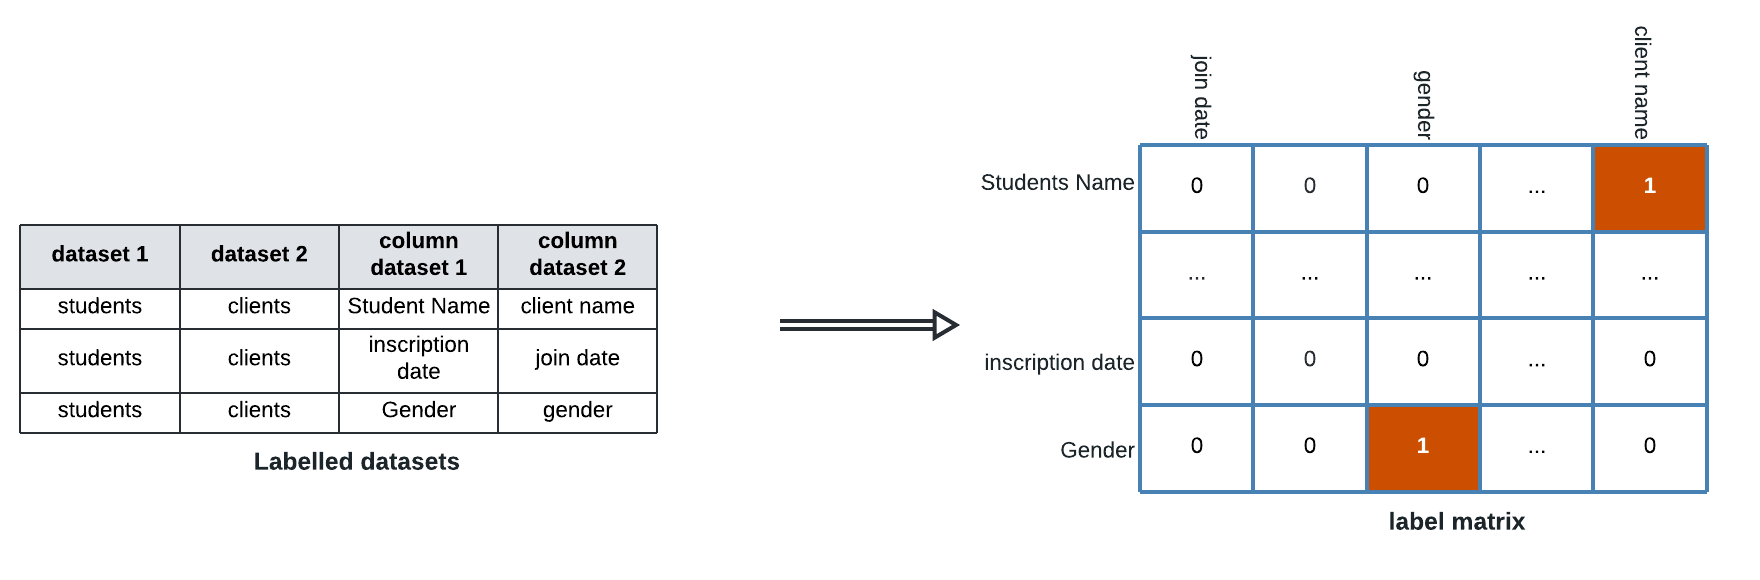
\includegraphics[width=\textwidth]{tests/labelled_entry.png}
    \caption{Label matrix generation from the labelled column similarities}
    \label{fig:label_matrix}
\end{figure}

\subfile{tests/01-embedding_metric.tex}

\subfile{tests/02-index_hp.tex}